Another algorithm for meta reinforcement learning is evolved policy gradient (EPG)\cite{epg}. Unlike meta gradient algorithm which focuses on learning the return function, EPG aims to learn a surrogate loss function $L_\phi = L_{\phi + \sigma\epsilon_i}$, which is parameterized by parameter $\phi$ along with a small Gaussian noise $\epsilon_i \sim \mathcal{N}(0, \mathbf{I})$ as perturbed terms.

\par
EPG contains an inner loop and an outer loop during its execution. In inner loop, the algorithm functions as normal policy gradient algorithm that tries to update parameter $\theta$ according to the following formula:

\[\theta^* = \argmin_\theta\EX_{\tau\thicksim\mathcal{M},\pi_\theta}[L_\phi(\pi_\theta,\tau)]\]

where $\theta^*$ is the updated parameter $\theta$, $\mathcal{M}$ is a sampled markov decision process, $\tau$ is an episode of $\mathcal{M}$ with horizon $\textit{H}$. The objective of the inner loop is to minimize the loss function $L_\phi$. In outer loop, the loss function parameter $\phi$ is updated as shown below:

\[\phi^* = \argmax_\phi\EX_{\mathcal{M}\thicksim p(\mathcal{M})}\EX_{\tau\thicksim\mathcal{M},\pi_{\theta^*}}[R_\tau]\]

where $p(\mathcal{M})$ is a distribution over MDPs, $\pi_{\theta^*}$ is the agent's policy trained with the loss function $L_\phi$ and $R_\tau = \sum_{t=0}^{H}\gamma^t{r_t}$ is the discounted episodic return of $\tau$. The goal of the outer loop is to achieve high expected returns in the MDP distribution.

\par
Pseudocode of EPG algorithm is shown below:
\begin{figure}[H]
	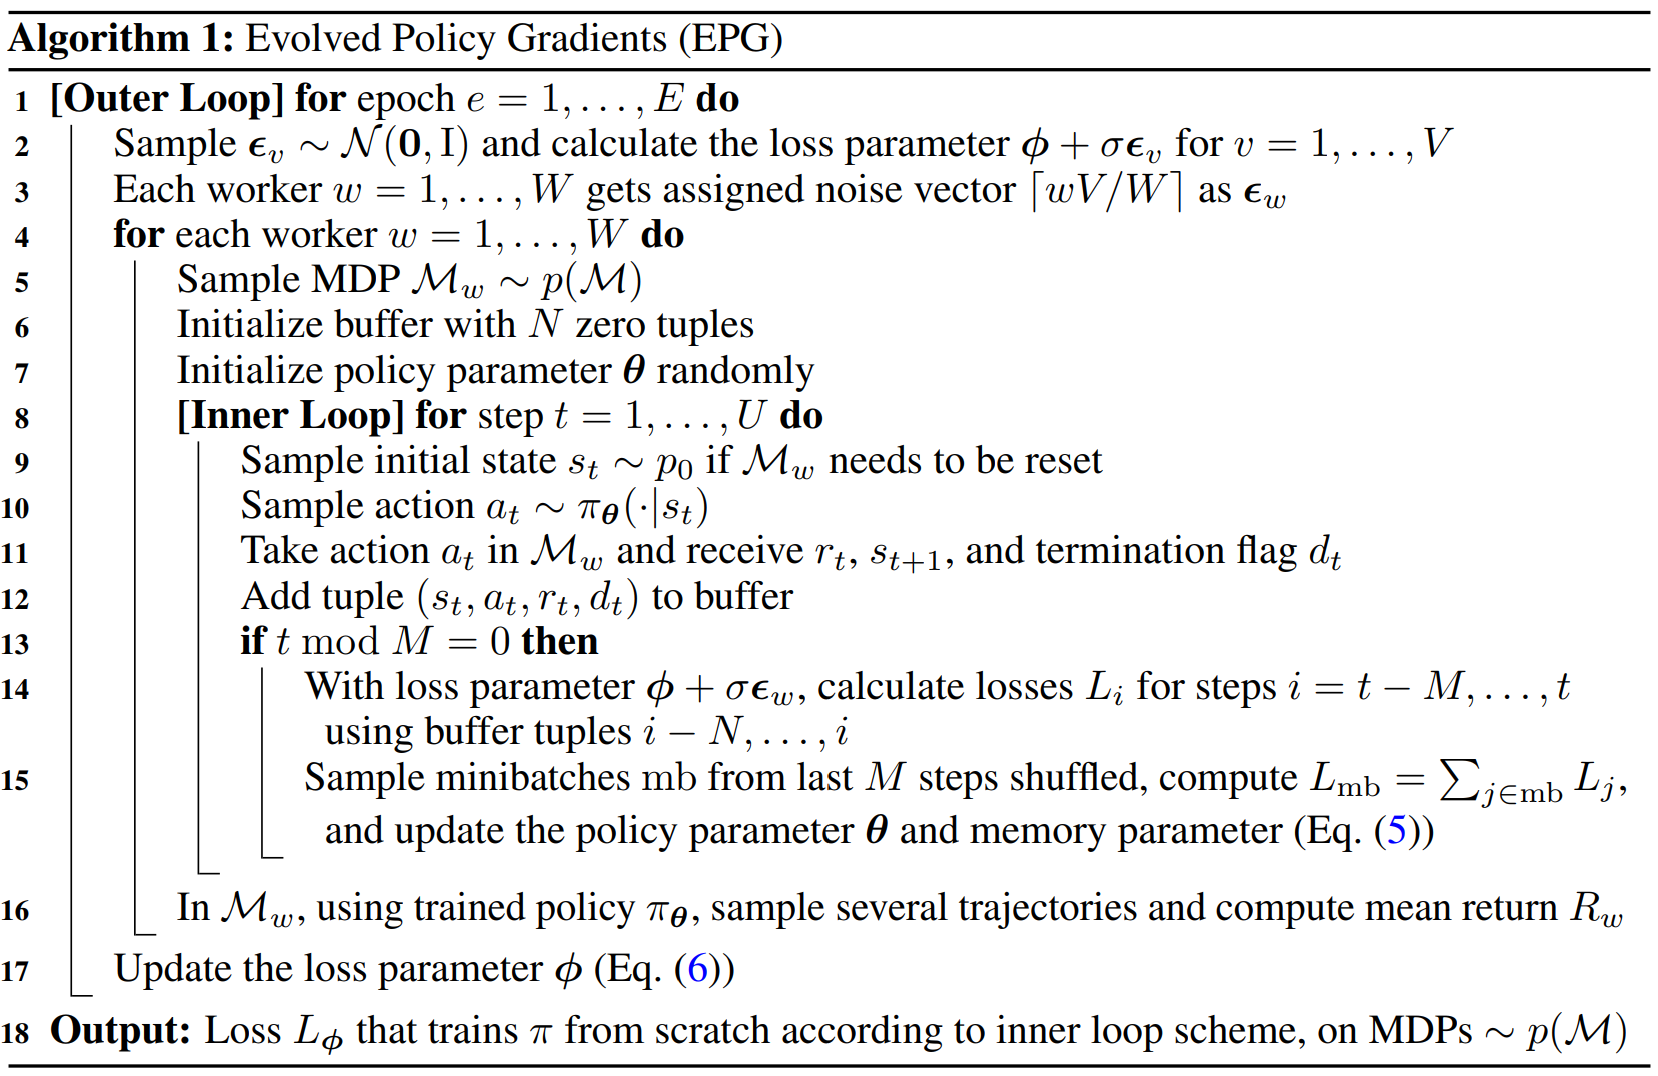
\includegraphics[scale=0.4]{epg.png}
	\centering
	\caption{EPG algorithm.}
	\label{epg}
\end{figure}

\par
The algorithm works as follows: Assumed that $\textit{W}$ workers are working in the inner loop. Then, at the beginning of each epoch in the outer loop, $\textit{V}$ multivariate normal vectors $\epsilon_v \in \mathcal{N}(0,I)$ of the same dimension as the loss function parameter $\phi$ are generated and assigned to $\textit{V}$ loss functions $L_\omega = L_{\phi+\delta\epsilon_v}$ respectively, with $\textit{v}$ being the $\textit{v}$-th generated perturbed parameters. 